\documentclass[]{article}
\usepackage{lmodern}
\usepackage{amssymb,amsmath}
\usepackage{ifxetex,ifluatex}
\usepackage{fixltx2e} % provides \textsubscript
\ifnum 0\ifxetex 1\fi\ifluatex 1\fi=0 % if pdftex
  \usepackage[T1]{fontenc}
  \usepackage[utf8]{inputenc}
\else % if luatex or xelatex
  \ifxetex
    \usepackage{mathspec}
  \else
    \usepackage{fontspec}
  \fi
  \defaultfontfeatures{Ligatures=TeX,Scale=MatchLowercase}
\fi
% use upquote if available, for straight quotes in verbatim environments
\IfFileExists{upquote.sty}{\usepackage{upquote}}{}
% use microtype if available
\IfFileExists{microtype.sty}{%
\usepackage{microtype}
\UseMicrotypeSet[protrusion]{basicmath} % disable protrusion for tt fonts
}{}
\usepackage[margin=1in]{geometry}
\usepackage{hyperref}
\hypersetup{unicode=true,
            pdftitle={Analysis of Attrition Data: Main factors that affect Employee Turnover},
            pdfauthor={Chaoshun Hu, Mahesh Kuklani, Rene Pineda},
            pdfborder={0 0 0},
            breaklinks=true}
\urlstyle{same}  % don't use monospace font for urls
\usepackage{color}
\usepackage{fancyvrb}
\newcommand{\VerbBar}{|}
\newcommand{\VERB}{\Verb[commandchars=\\\{\}]}
\DefineVerbatimEnvironment{Highlighting}{Verbatim}{commandchars=\\\{\}}
% Add ',fontsize=\small' for more characters per line
\usepackage{framed}
\definecolor{shadecolor}{RGB}{248,248,248}
\newenvironment{Shaded}{\begin{snugshade}}{\end{snugshade}}
\newcommand{\KeywordTok}[1]{\textcolor[rgb]{0.13,0.29,0.53}{\textbf{{#1}}}}
\newcommand{\DataTypeTok}[1]{\textcolor[rgb]{0.13,0.29,0.53}{{#1}}}
\newcommand{\DecValTok}[1]{\textcolor[rgb]{0.00,0.00,0.81}{{#1}}}
\newcommand{\BaseNTok}[1]{\textcolor[rgb]{0.00,0.00,0.81}{{#1}}}
\newcommand{\FloatTok}[1]{\textcolor[rgb]{0.00,0.00,0.81}{{#1}}}
\newcommand{\ConstantTok}[1]{\textcolor[rgb]{0.00,0.00,0.00}{{#1}}}
\newcommand{\CharTok}[1]{\textcolor[rgb]{0.31,0.60,0.02}{{#1}}}
\newcommand{\SpecialCharTok}[1]{\textcolor[rgb]{0.00,0.00,0.00}{{#1}}}
\newcommand{\StringTok}[1]{\textcolor[rgb]{0.31,0.60,0.02}{{#1}}}
\newcommand{\VerbatimStringTok}[1]{\textcolor[rgb]{0.31,0.60,0.02}{{#1}}}
\newcommand{\SpecialStringTok}[1]{\textcolor[rgb]{0.31,0.60,0.02}{{#1}}}
\newcommand{\ImportTok}[1]{{#1}}
\newcommand{\CommentTok}[1]{\textcolor[rgb]{0.56,0.35,0.01}{\textit{{#1}}}}
\newcommand{\DocumentationTok}[1]{\textcolor[rgb]{0.56,0.35,0.01}{\textbf{\textit{{#1}}}}}
\newcommand{\AnnotationTok}[1]{\textcolor[rgb]{0.56,0.35,0.01}{\textbf{\textit{{#1}}}}}
\newcommand{\CommentVarTok}[1]{\textcolor[rgb]{0.56,0.35,0.01}{\textbf{\textit{{#1}}}}}
\newcommand{\OtherTok}[1]{\textcolor[rgb]{0.56,0.35,0.01}{{#1}}}
\newcommand{\FunctionTok}[1]{\textcolor[rgb]{0.00,0.00,0.00}{{#1}}}
\newcommand{\VariableTok}[1]{\textcolor[rgb]{0.00,0.00,0.00}{{#1}}}
\newcommand{\ControlFlowTok}[1]{\textcolor[rgb]{0.13,0.29,0.53}{\textbf{{#1}}}}
\newcommand{\OperatorTok}[1]{\textcolor[rgb]{0.81,0.36,0.00}{\textbf{{#1}}}}
\newcommand{\BuiltInTok}[1]{{#1}}
\newcommand{\ExtensionTok}[1]{{#1}}
\newcommand{\PreprocessorTok}[1]{\textcolor[rgb]{0.56,0.35,0.01}{\textit{{#1}}}}
\newcommand{\AttributeTok}[1]{\textcolor[rgb]{0.77,0.63,0.00}{{#1}}}
\newcommand{\RegionMarkerTok}[1]{{#1}}
\newcommand{\InformationTok}[1]{\textcolor[rgb]{0.56,0.35,0.01}{\textbf{\textit{{#1}}}}}
\newcommand{\WarningTok}[1]{\textcolor[rgb]{0.56,0.35,0.01}{\textbf{\textit{{#1}}}}}
\newcommand{\AlertTok}[1]{\textcolor[rgb]{0.94,0.16,0.16}{{#1}}}
\newcommand{\ErrorTok}[1]{\textcolor[rgb]{0.64,0.00,0.00}{\textbf{{#1}}}}
\newcommand{\NormalTok}[1]{{#1}}
\usepackage{graphicx,grffile}
\makeatletter
\def\maxwidth{\ifdim\Gin@nat@width>\linewidth\linewidth\else\Gin@nat@width\fi}
\def\maxheight{\ifdim\Gin@nat@height>\textheight\textheight\else\Gin@nat@height\fi}
\makeatother
% Scale images if necessary, so that they will not overflow the page
% margins by default, and it is still possible to overwrite the defaults
% using explicit options in \includegraphics[width, height, ...]{}
\setkeys{Gin}{width=\maxwidth,height=\maxheight,keepaspectratio}
\IfFileExists{parskip.sty}{%
\usepackage{parskip}
}{% else
\setlength{\parindent}{0pt}
\setlength{\parskip}{6pt plus 2pt minus 1pt}
}
\setlength{\emergencystretch}{3em}  % prevent overfull lines
\providecommand{\tightlist}{%
  \setlength{\itemsep}{0pt}\setlength{\parskip}{0pt}}
\setcounter{secnumdepth}{0}
% Redefines (sub)paragraphs to behave more like sections
\ifx\paragraph\undefined\else
\let\oldparagraph\paragraph
\renewcommand{\paragraph}[1]{\oldparagraph{#1}\mbox{}}
\fi
\ifx\subparagraph\undefined\else
\let\oldsubparagraph\subparagraph
\renewcommand{\subparagraph}[1]{\oldsubparagraph{#1}\mbox{}}
\fi

%%% Use protect on footnotes to avoid problems with footnotes in titles
\let\rmarkdownfootnote\footnote%
\def\footnote{\protect\rmarkdownfootnote}

%%% Change title format to be more compact
\usepackage{titling}

% Create subtitle command for use in maketitle
\newcommand{\subtitle}[1]{
  \posttitle{
    \begin{center}\large#1\end{center}
    }
}

\setlength{\droptitle}{-2em}
  \title{Analysis of Attrition Data: Main factors that affect Employee Turnover}
  \pretitle{\vspace{\droptitle}\centering\huge}
  \posttitle{\par}
  \author{Chaoshun Hu, Mahesh Kuklani, Rene Pineda}
  \preauthor{\centering\large\emph}
  \postauthor{\par}
  \predate{\centering\large\emph}
  \postdate{\par}
  \date{August 7, 2018}


\begin{document}
\maketitle

\subsection{Introduction}\label{introduction}

Voluntary attrition occurs when an employee leaves a company of his or
her own accord. This can occur when employees leave their current
positions for another job, leave the workforce entirely, or retire. The
reasons for leaving a company can vary from personal reasons, such as
desiring career advancement or moving to a different city, to
company-based reasons, such as an unwanted change in company structure
or management.

A high turnover rate typically means working conditions are not optimal,
pay is below market average, or staffers are not well trained.
Concurrently, a low turnover rate is indicative of a work environment
where staffers feel appreciated, work as a team, have room to move up
the corporate ladder, and are satisfied with their jobs.

Attrition rates vary widely accross industries. The following tables
show attrition rates in the United States:

\begin{figure}[htbp]
\centering
\includegraphics{E:/Bibliotecas/Documents/Data\%20Science/SMU/MSDS\%206306\%20Doing\%20Data\%20Science/Project\%202/Attrition\%20Statistics.jpg}
\caption{}
\end{figure}

Employee attrition statistics have worsened in recent years, after years
of recovery over the recesion of 2008:

\begin{figure}[htbp]
\centering
\includegraphics{E:/Bibliotecas/Documents/Data\%20Science/SMU/MSDS\%206306\%20Doing\%20Data\%20Science/Project\%202/Historical\%20Attrition.jpg}
\caption{}
\end{figure}

Source: CompData's 2016 edition of their annual BenchmarkPro Survey

Companies usually would like to decrease their voluntary turnover rates
due to numerous unfavorable impacts: * Overall poor company performance
* Low employee morale * Monetary costs (severance payments, cost of
re-hiring and re-training) * Money invested in the employees that leave
the company can't be recovered * The decrease in the workforce causes
remaining employees to work on the slack left behind- mostly performing
the task they are not completely trained to perform or are not the best
suited * The situation may get out of control and lead to mass exit of
employees, disabling the ability of the company to perform at a high
level.

In order to deal with employee attrition and deal with its negative
impacts, it is important to know about the most important causes of
Attrition. The purpose of this analysis is to try to dilucidate what are
the most important factors that contribute to attrition, amongst the
many factors that affect an employee's environment and satisfaction.
Once these factors are determined, a company can take actions to control
them.

\subsubsection{2. Loading and cleaning the
data}\label{loading-and-cleaning-the-data}

\textbf{a Read the csv into R and take a look at the data set. Output
how many rows and columns the data.frame is.}

\begin{Shaded}
\begin{Highlighting}[]
\KeywordTok{dim}\NormalTok{(talentManage)}
\end{Highlighting}
\end{Shaded}

\begin{verbatim}
## [1] 1470   35
\end{verbatim}

The \texttt{talentManage} data frame has 1470 rows and 35 columns.

\textbf{b The column names are either too much or not enough. Change the
column names so that they do not have spaces, underscores, slashes, and
the like. All column names should be under 12 characters. Make sure
you're updating your codebook with information on the tidied data set as
well.}

We use an R function to automatically abbreviate the variable names:

\begin{Shaded}
\begin{Highlighting}[]
\CommentTok{#List column names}
\KeywordTok{colnames}\NormalTok{(talentManage)}
\end{Highlighting}
\end{Shaded}

\begin{verbatim}
##  [1] "Age"                      "Attrition"               
##  [3] "BusinessTravel"           "DailyRate"               
##  [5] "Department"               "DistanceFromHome"        
##  [7] "Education"                "EducationField"          
##  [9] "EmployeeCount"            "EmployeeNumber"          
## [11] "EnvironmentSatisfaction"  "Gender"                  
## [13] "HourlyRate"               "JobInvolvement"          
## [15] "JobLevel"                 "JobRole"                 
## [17] "JobSatisfaction"          "MaritalStatus"           
## [19] "MonthlyIncome"            "MonthlyRate"             
## [21] "NumCompaniesWorked"       "Over18"                  
## [23] "OverTime"                 "PercentSalaryHike"       
## [25] "PerformanceRating"        "RelationshipSatisfaction"
## [27] "StandardHours"            "StockOptionLevel"        
## [29] "TotalWorkingYears"        "TrainingTimesLastYear"   
## [31] "WorkLifeBalance"          "YearsAtCompany"          
## [33] "YearsInCurrentRole"       "YearsSinceLastPromotion" 
## [35] "YearsWithCurrManager"
\end{verbatim}

\begin{Shaded}
\begin{Highlighting}[]
\CommentTok{#Abbreviate column names}
\KeywordTok{colnames}\NormalTok{(talentManage)=}\KeywordTok{abbreviate}\NormalTok{(}\KeywordTok{colnames}\NormalTok{(talentManage), }\DataTypeTok{method=}\KeywordTok{c}\NormalTok{(}\StringTok{"both.sides"}\NormalTok{),}\DataTypeTok{minlength =} \DecValTok{11}\NormalTok{)}
\end{Highlighting}
\end{Shaded}

We will now list the column names again and count the characters to
confirm confirm that none exceeds the 12-character limit

\begin{Shaded}
\begin{Highlighting}[]
\NormalTok{columns <-}\StringTok{ }\KeywordTok{colnames}\NormalTok{(talentManage)}
\NormalTok{columns}
\end{Highlighting}
\end{Shaded}

\begin{verbatim}
##  [1] "Age"         "Attrition"   "BusinssTrvl" "DailyRate"   "Department" 
##  [6] "DistncFrmHm" "Education"   "EducatinFld" "EmployeeCnt" "EmployeNmbr"
## [11] "EnvrnmntSts" "Gender"      "HourlyRate"  "JobInvlvmnt" "JobLevel"   
## [16] "JobRole"     "JobSatsfctn" "MaritalStts" "MonthlyIncm" "MonthlyRate"
## [21] "NmCmpnsWrkd" "Over18"      "OverTime"    "PrcntSlryHk" "PrfrmncRtng"
## [26] "RltnshpStsf" "StandardHrs" "StckOptnLvl" "TtlWrkngYrs" "TrnngTmsLsY"
## [31] "WorkLifBlnc" "YersAtCmpny" "YrsInCrrntR" "YrsSncLstPr" "YrsWthCrrMn"
\end{verbatim}

\begin{Shaded}
\begin{Highlighting}[]
\KeywordTok{sapply}\NormalTok{(columns, nchar)}
\end{Highlighting}
\end{Shaded}

\begin{verbatim}
##         Age   Attrition BusinssTrvl   DailyRate  Department DistncFrmHm 
##           3           9          11           9          10          11 
##   Education EducatinFld EmployeeCnt EmployeNmbr EnvrnmntSts      Gender 
##           9          11          11          11          11           6 
##  HourlyRate JobInvlvmnt    JobLevel     JobRole JobSatsfctn MaritalStts 
##          10          11           8           7          11          11 
## MonthlyIncm MonthlyRate NmCmpnsWrkd      Over18    OverTime PrcntSlryHk 
##          11          11          11           6           8          11 
## PrfrmncRtng RltnshpStsf StandardHrs StckOptnLvl TtlWrkngYrs TrnngTmsLsY 
##          11          11          11          11          11          11 
## WorkLifBlnc YersAtCmpny YrsInCrrntR YrsSncLstPr YrsWthCrrMn 
##          11          11          11          11          11
\end{verbatim}

\textbf{c. Some columns are, due to Qualtrics, malfunctioning. }

\textbf{d. Make sure your columns are the proper data types (i.e.,
numeric, character, etc.). If they are incorrect, convert them.}

\begin{Shaded}
\begin{Highlighting}[]
\CommentTok{#Check the 'class' of each variable column}
\KeywordTok{lapply}\NormalTok{(talentManage, class)}
\end{Highlighting}
\end{Shaded}

\begin{verbatim}
## $Age
## [1] "integer"
## 
## $Attrition
## [1] "factor"
## 
## $BusinssTrvl
## [1] "factor"
## 
## $DailyRate
## [1] "integer"
## 
## $Department
## [1] "factor"
## 
## $DistncFrmHm
## [1] "integer"
## 
## $Education
## [1] "integer"
## 
## $EducatinFld
## [1] "factor"
## 
## $EmployeeCnt
## [1] "integer"
## 
## $EmployeNmbr
## [1] "integer"
## 
## $EnvrnmntSts
## [1] "integer"
## 
## $Gender
## [1] "factor"
## 
## $HourlyRate
## [1] "integer"
## 
## $JobInvlvmnt
## [1] "integer"
## 
## $JobLevel
## [1] "integer"
## 
## $JobRole
## [1] "factor"
## 
## $JobSatsfctn
## [1] "integer"
## 
## $MaritalStts
## [1] "factor"
## 
## $MonthlyIncm
## [1] "integer"
## 
## $MonthlyRate
## [1] "integer"
## 
## $NmCmpnsWrkd
## [1] "integer"
## 
## $Over18
## [1] "factor"
## 
## $OverTime
## [1] "factor"
## 
## $PrcntSlryHk
## [1] "integer"
## 
## $PrfrmncRtng
## [1] "integer"
## 
## $RltnshpStsf
## [1] "integer"
## 
## $StandardHrs
## [1] "integer"
## 
## $StckOptnLvl
## [1] "integer"
## 
## $TtlWrkngYrs
## [1] "integer"
## 
## $TrnngTmsLsY
## [1] "integer"
## 
## $WorkLifBlnc
## [1] "integer"
## 
## $YersAtCmpny
## [1] "integer"
## 
## $YrsInCrrntR
## [1] "integer"
## 
## $YrsSncLstPr
## [1] "integer"
## 
## $YrsWthCrrMn
## [1] "integer"
\end{verbatim}

\begin{Shaded}
\begin{Highlighting}[]
\CommentTok{#Recode variables from 'numeric' to 'factor'}
\NormalTok{talentManage[,}\DecValTok{7}\NormalTok{] <-}\StringTok{ }\KeywordTok{factor}\NormalTok{(talentManage[,}\DecValTok{7}\NormalTok{], }\DataTypeTok{labels =} \KeywordTok{c}\NormalTok{(}\StringTok{"Below College"}\NormalTok{, }\StringTok{"College"}\NormalTok{, }\StringTok{"Bachelor"}\NormalTok{, }\StringTok{"Master"}\NormalTok{, }\StringTok{"Doctor"}\NormalTok{), }\DataTypeTok{ordered =} \OtherTok{TRUE}\NormalTok{)}
\NormalTok{talentManage[,}\DecValTok{11}\NormalTok{] <-}\StringTok{ }\KeywordTok{factor}\NormalTok{(talentManage[,}\DecValTok{11}\NormalTok{], }\DataTypeTok{labels =} \KeywordTok{c}\NormalTok{(}\StringTok{'Low'}\NormalTok{, }\StringTok{'Medium'}\NormalTok{, }\StringTok{'High'}\NormalTok{, }\StringTok{'Very High'}\NormalTok{), }\DataTypeTok{ordered =} \OtherTok{TRUE}\NormalTok{)}
\NormalTok{talentManage[,}\DecValTok{14}\NormalTok{] <-}\StringTok{ }\KeywordTok{factor}\NormalTok{(talentManage[,}\DecValTok{14}\NormalTok{], }\DataTypeTok{labels =} \KeywordTok{c}\NormalTok{(}\StringTok{'Low'}\NormalTok{, }\StringTok{'Medium'}\NormalTok{, }\StringTok{'High'}\NormalTok{, }\StringTok{'Very High'}\NormalTok{), }\DataTypeTok{ordered =} \OtherTok{TRUE}\NormalTok{)}
\NormalTok{talentManage[,}\DecValTok{17}\NormalTok{] <-}\StringTok{ }\KeywordTok{factor}\NormalTok{(talentManage[,}\DecValTok{17}\NormalTok{], }\DataTypeTok{labels =} \KeywordTok{c}\NormalTok{(}\StringTok{'Low'}\NormalTok{, }\StringTok{'Medium'}\NormalTok{, }\StringTok{'High'}\NormalTok{, }\StringTok{'Very High'}\NormalTok{), }\DataTypeTok{ordered =} \OtherTok{TRUE}\NormalTok{)}
\NormalTok{talentManage[,}\DecValTok{25}\NormalTok{] <-}\StringTok{ }\KeywordTok{factor}\NormalTok{(talentManage[,}\DecValTok{25}\NormalTok{], }\DataTypeTok{labels =} \KeywordTok{c}\NormalTok{(}\StringTok{'Excellent'}\NormalTok{, }\StringTok{'Outstanding'}\NormalTok{), }\DataTypeTok{ordered =} \OtherTok{TRUE}\NormalTok{)}
\NormalTok{talentManage[,}\DecValTok{26}\NormalTok{] <-}\StringTok{ }\KeywordTok{factor}\NormalTok{(talentManage[,}\DecValTok{26}\NormalTok{], }\DataTypeTok{labels =} \KeywordTok{c}\NormalTok{(}\StringTok{'Low'}\NormalTok{, }\StringTok{'Medium'}\NormalTok{, }\StringTok{'High'}\NormalTok{, }\StringTok{'Very High'}\NormalTok{), }\DataTypeTok{ordered =} \OtherTok{TRUE}\NormalTok{)}
\NormalTok{talentManage[,}\DecValTok{31}\NormalTok{] <-}\StringTok{ }\KeywordTok{factor}\NormalTok{(talentManage[,}\DecValTok{31}\NormalTok{], }\DataTypeTok{labels =} \KeywordTok{c}\NormalTok{(}\StringTok{'Bad'}\NormalTok{, }\StringTok{'Good'}\NormalTok{, }\StringTok{'Better'}\NormalTok{, }\StringTok{'Best'}\NormalTok{), }\DataTypeTok{ordered =} \OtherTok{TRUE}\NormalTok{)}
\NormalTok{talentManage[,}\DecValTok{15}\NormalTok{] <-}\StringTok{ }\KeywordTok{factor}\NormalTok{(talentManage[,}\DecValTok{15}\NormalTok{], }\DataTypeTok{ordered =} \OtherTok{TRUE}\NormalTok{)}
\NormalTok{talentManage[,}\DecValTok{28}\NormalTok{] <-}\StringTok{ }\KeywordTok{factor}\NormalTok{(talentManage[,}\DecValTok{28}\NormalTok{])}

\CommentTok{#Perform an additional recoding: divide the "Years with Current Manager" variable into three groups}
\NormalTok{talentManage[,}\DecValTok{35}\NormalTok{] <-}\StringTok{ }\KeywordTok{cut}\NormalTok{(talentManage[,}\DecValTok{35}\NormalTok{], }\DataTypeTok{breaks =} \KeywordTok{c}\NormalTok{(}\DecValTok{0}\NormalTok{,}\DecValTok{5}\NormalTok{,}\DecValTok{10}\NormalTok{,}\DecValTok{17}\NormalTok{), }\DataTypeTok{labels =} \KeywordTok{c}\NormalTok{(}\StringTok{"0-5"}\NormalTok{, }\StringTok{"6-10"}\NormalTok{, }\StringTok{"More than 10"}\NormalTok{), }\DataTypeTok{right =} \OtherTok{TRUE}\NormalTok{, }\DataTypeTok{include.lowest =} \OtherTok{TRUE}\NormalTok{, }\DataTypeTok{ordered_result =} \OtherTok{TRUE}\NormalTok{)}

\CommentTok{#Check that all variables have the correct 'class'}
\KeywordTok{str}\NormalTok{(talentManage)}
\end{Highlighting}
\end{Shaded}

\begin{verbatim}
## 'data.frame':    1470 obs. of  35 variables:
##  $ Age        : int  41 49 37 33 27 32 59 30 38 36 ...
##  $ Attrition  : Factor w/ 2 levels "No","Yes": 2 1 2 1 1 1 1 1 1 1 ...
##  $ BusinssTrvl: Factor w/ 3 levels "Non-Travel","Travel_Frequently",..: 3 2 3 2 3 2 3 3 2 3 ...
##  $ DailyRate  : int  1102 279 1373 1392 591 1005 1324 1358 216 1299 ...
##  $ Department : Factor w/ 3 levels "Human Resources",..: 3 2 2 2 2 2 2 2 2 2 ...
##  $ DistncFrmHm: int  1 8 2 3 2 2 3 24 23 27 ...
##  $ Education  : Ord.factor w/ 5 levels "Below College"<..: 2 1 2 4 1 2 3 1 3 3 ...
##  $ EducatinFld: Factor w/ 6 levels "Human Resources",..: 2 2 5 2 4 2 4 2 2 4 ...
##  $ EmployeeCnt: int  1 1 1 1 1 1 1 1 1 1 ...
##  $ EmployeNmbr: int  1 2 4 5 7 8 10 11 12 13 ...
##  $ EnvrnmntSts: Ord.factor w/ 4 levels "Low"<"Medium"<..: 2 3 4 4 1 4 3 4 4 3 ...
##  $ Gender     : Factor w/ 2 levels "Female","Male": 1 2 2 1 2 2 1 2 2 2 ...
##  $ HourlyRate : int  94 61 92 56 40 79 81 67 44 94 ...
##  $ JobInvlvmnt: Ord.factor w/ 4 levels "Low"<"Medium"<..: 3 2 2 3 3 3 4 3 2 3 ...
##  $ JobLevel   : Ord.factor w/ 5 levels "1"<"2"<"3"<"4"<..: 2 2 1 1 1 1 1 1 3 2 ...
##  $ JobRole    : Factor w/ 9 levels "Healthcare Representative",..: 8 7 3 7 3 3 3 3 5 1 ...
##  $ JobSatsfctn: Ord.factor w/ 4 levels "Low"<"Medium"<..: 4 2 3 3 2 4 1 3 3 3 ...
##  $ MaritalStts: Factor w/ 3 levels "Divorced","Married",..: 3 2 3 2 2 3 2 1 3 2 ...
##  $ MonthlyIncm: int  5993 5130 2090 2909 3468 3068 2670 2693 9526 5237 ...
##  $ MonthlyRate: int  19479 24907 2396 23159 16632 11864 9964 13335 8787 16577 ...
##  $ NmCmpnsWrkd: int  8 1 6 1 9 0 4 1 0 6 ...
##  $ Over18     : Factor w/ 1 level "Y": 1 1 1 1 1 1 1 1 1 1 ...
##  $ OverTime   : Factor w/ 2 levels "No","Yes": 2 1 2 2 1 1 2 1 1 1 ...
##  $ PrcntSlryHk: int  11 23 15 11 12 13 20 22 21 13 ...
##  $ PrfrmncRtng: Ord.factor w/ 2 levels "Excellent"<"Outstanding": 1 2 1 1 1 1 2 2 2 1 ...
##  $ RltnshpStsf: Ord.factor w/ 4 levels "Low"<"Medium"<..: 1 4 2 3 4 3 1 2 2 2 ...
##  $ StandardHrs: int  80 80 80 80 80 80 80 80 80 80 ...
##  $ StckOptnLvl: Factor w/ 4 levels "0","1","2","3": 1 2 1 1 2 1 4 2 1 3 ...
##  $ TtlWrkngYrs: int  8 10 7 8 6 8 12 1 10 17 ...
##  $ TrnngTmsLsY: int  0 3 3 3 3 2 3 2 2 3 ...
##  $ WorkLifBlnc: Ord.factor w/ 4 levels "Bad"<"Good"<"Better"<..: 1 3 3 3 3 2 2 3 3 2 ...
##  $ YersAtCmpny: int  6 10 0 8 2 7 1 1 9 7 ...
##  $ YrsInCrrntR: int  4 7 0 7 2 7 0 0 7 7 ...
##  $ YrsSncLstPr: int  0 1 0 3 2 3 0 0 1 7 ...
##  $ YrsWthCrrMn: Ord.factor w/ 3 levels "0-5"<"6-10"<"More than 10": 1 2 1 1 1 2 1 1 2 2 ...
\end{verbatim}

\subsubsection{3. Preliminary Analysis}\label{preliminary-analysis}

\textbf{a Remove all observations where the participant is under age 18.
No further analysis of underage individuals is permitted by your client.
Remove any other age outliers as you see fit, but be sure to tell what
you're doing and why.}

First we apply a function to check whether there are participants under
age 18:

\begin{Shaded}
\begin{Highlighting}[]
\CommentTok{#Check every value of the 'Age' variable to see whether it is smaller than 18}
\KeywordTok{summary}\NormalTok{(}\KeywordTok{sapply}\NormalTok{(talentManage$Age, function(x) x <}\StringTok{ }\DecValTok{18}\NormalTok{))}
\end{Highlighting}
\end{Shaded}

\begin{verbatim}
##    Mode   FALSE    NA's 
## logical    1470       0
\end{verbatim}

There are no participants under age 18.

Regarding outliers, we might want to remove participants who have passed
the age of retirement (65 years old, although this has increased due to
SS ammendments) and that might be having a negative impact in attrition
rates, because attrition would be disproportionately high in this group.
We can check this in the data

\begin{Shaded}
\begin{Highlighting}[]
\CommentTok{#Check every value of the 'Age' variable to see whether it is smaller than 18}
\KeywordTok{summary}\NormalTok{(}\KeywordTok{sapply}\NormalTok{(talentManage$Age, function(x) x >=}\StringTok{ }\DecValTok{65}\NormalTok{))}
\end{Highlighting}
\end{Shaded}

\begin{verbatim}
##    Mode   FALSE    NA's 
## logical    1470       0
\end{verbatim}

\begin{Shaded}
\begin{Highlighting}[]
\NormalTok{retirement <-}\StringTok{ }\KeywordTok{subset}\NormalTok{(talentManage$Age, talentManage$Age >=}\DecValTok{60}\NormalTok{)}
\NormalTok{retirement  }
\end{Highlighting}
\end{Shaded}

\begin{verbatim}
## [1] 60 60 60 60 60
\end{verbatim}

We do not have instances of people 65 years old or older, and only a
handful of participants are 60 years old. We proceed without eliminating
any data points.

\textbf{b Please provide (in table format or similar), descriptive
statistics on at least 7 variables (age, Income, etc.). Create a simple
histogram for two of them. Comment on the shape of the distribution in
your markdown.} \#Summary tables

\begin{Shaded}
\begin{Highlighting}[]
\KeywordTok{options}\NormalTok{(}\DataTypeTok{qwraps2_markup =} \StringTok{"markdown"}\NormalTok{)}
\NormalTok{summary_numeric <-}\StringTok{ }\KeywordTok{with}\NormalTok{(talentManage,}
                \KeywordTok{list}\NormalTok{(}\StringTok{"Age"} \NormalTok{=}\StringTok{ }\KeywordTok{tab_summary}\NormalTok{(Age)[}\KeywordTok{c}\NormalTok{(}\DecValTok{1}\NormalTok{,}\DecValTok{4}\NormalTok{,}\DecValTok{2}\NormalTok{,}\DecValTok{3}\NormalTok{)],}
                     \StringTok{"Monthly Income"} \NormalTok{=}\StringTok{ }\KeywordTok{tab_summary}\NormalTok{(MonthlyIncm)[}\KeywordTok{c}\NormalTok{(}\DecValTok{1}\NormalTok{,}\DecValTok{4}\NormalTok{,}\DecValTok{2}\NormalTok{,}\DecValTok{3}\NormalTok{)],}
                     \StringTok{"Distance From Home"} \NormalTok{=}\StringTok{ }\KeywordTok{tab_summary}\NormalTok{(DistncFrmHm)[}\KeywordTok{c}\NormalTok{(}\DecValTok{1}\NormalTok{,}\DecValTok{4}\NormalTok{,}\DecValTok{2}\NormalTok{,}\DecValTok{3}\NormalTok{)],}
                     \StringTok{"Number of Companies Worked In"} \NormalTok{=}\StringTok{ }\KeywordTok{tab_summary}\NormalTok{(NmCmpnsWrkd)[}\KeywordTok{c}\NormalTok{(}\DecValTok{1}\NormalTok{,}\DecValTok{4}\NormalTok{,}\DecValTok{2}\NormalTok{,}\DecValTok{3}\NormalTok{)],}
                     \StringTok{"Percent Salary Raise"} \NormalTok{=}\StringTok{ }\KeywordTok{tab_summary}\NormalTok{(PrcntSlryHk)[}\KeywordTok{c}\NormalTok{(}\DecValTok{1}\NormalTok{,}\DecValTok{4}\NormalTok{,}\DecValTok{2}\NormalTok{,}\DecValTok{3}\NormalTok{)],}
                     \StringTok{"Total working Years"} \NormalTok{=}\StringTok{ }\KeywordTok{tab_summary}\NormalTok{(TtlWrkngYrs)[}\KeywordTok{c}\NormalTok{(}\DecValTok{1}\NormalTok{,}\DecValTok{4}\NormalTok{,}\DecValTok{2}\NormalTok{,}\DecValTok{3}\NormalTok{)],}
                     \StringTok{"Years at Company"} \NormalTok{=}\StringTok{ }\KeywordTok{tab_summary}\NormalTok{(YersAtCmpny)[}\KeywordTok{c}\NormalTok{(}\DecValTok{1}\NormalTok{,}\DecValTok{4}\NormalTok{,}\DecValTok{2}\NormalTok{,}\DecValTok{3}\NormalTok{)]))}
                     
\KeywordTok{summary}\NormalTok{(}\KeywordTok{sapply}\NormalTok{(talentManage$Age, function(x) x <}\StringTok{ }\DecValTok{18}\NormalTok{))}
\end{Highlighting}
\end{Shaded}

\begin{verbatim}
##    Mode   FALSE    NA's 
## logical    1470       0
\end{verbatim}

\begin{Shaded}
\begin{Highlighting}[]
\NormalTok{table_numeric <-}\StringTok{ }\KeywordTok{summary_table}\NormalTok{(talentManage, summary_numeric)}
\NormalTok{table_numeric}
\end{Highlighting}
\end{Shaded}

\begin{verbatim}
## 
## 
## |                                  |talentManage (N = 1470)       |
## |:---------------------------------|:-----------------------------|
## |**Age**                           |&nbsp;&nbsp;                  |
## |&nbsp;&nbsp; min                  |18                            |
## |&nbsp;&nbsp; max                  |60                            |
## |&nbsp;&nbsp; median (IQR)         |36.00 (30.00, 43.00)          |
## |&nbsp;&nbsp; mean (sd)            |36.92 &plusmn; 9.14           |
## |**Monthly Income**                |&nbsp;&nbsp;                  |
## |&nbsp;&nbsp; min                  |1009                          |
## |&nbsp;&nbsp; max                  |19999                         |
## |&nbsp;&nbsp; median (IQR)         |4,919.00 (2,911.00, 8,379.00) |
## |&nbsp;&nbsp; mean (sd)            |6,502.93 &plusmn; 4,707.96    |
## |**Distance From Home**            |&nbsp;&nbsp;                  |
## |&nbsp;&nbsp; min                  |1                             |
## |&nbsp;&nbsp; max                  |29                            |
## |&nbsp;&nbsp; median (IQR)         |7.00 (2.00, 14.00)            |
## |&nbsp;&nbsp; mean (sd)            |9.19 &plusmn; 8.11            |
## |**Number of Companies Worked In** |&nbsp;&nbsp;                  |
## |&nbsp;&nbsp; min                  |0                             |
## |&nbsp;&nbsp; max                  |9                             |
## |&nbsp;&nbsp; median (IQR)         |2.00 (1.00, 4.00)             |
## |&nbsp;&nbsp; mean (sd)            |2.69 &plusmn; 2.50            |
## |**Percent Salary Raise**          |&nbsp;&nbsp;                  |
## |&nbsp;&nbsp; min                  |11                            |
## |&nbsp;&nbsp; max                  |25                            |
## |&nbsp;&nbsp; median (IQR)         |14.00 (12.00, 18.00)          |
## |&nbsp;&nbsp; mean (sd)            |15.21 &plusmn; 3.66           |
## |**Total working Years**           |&nbsp;&nbsp;                  |
## |&nbsp;&nbsp; min                  |0                             |
## |&nbsp;&nbsp; max                  |40                            |
## |&nbsp;&nbsp; median (IQR)         |10.00 (6.00, 15.00)           |
## |&nbsp;&nbsp; mean (sd)            |11.28 &plusmn; 7.78           |
## |**Years at Company**              |&nbsp;&nbsp;                  |
## |&nbsp;&nbsp; min                  |0                             |
## |&nbsp;&nbsp; max                  |40                            |
## |&nbsp;&nbsp; median (IQR)         |5.00 (3.00, 9.00)             |
## |&nbsp;&nbsp; mean (sd)            |7.01 &plusmn; 6.13            |
\end{verbatim}

\begin{Shaded}
\begin{Highlighting}[]
\CommentTok{#Create the required histograms}
\KeywordTok{ggplot}\NormalTok{(}\DataTypeTok{data =} \NormalTok{talentManage, }\DataTypeTok{mapping =} \KeywordTok{aes}\NormalTok{(Age)) +}
\StringTok{  }\KeywordTok{geom_histogram}\NormalTok{(}\DataTypeTok{binwidth =} \DecValTok{5}\NormalTok{, }\DataTypeTok{color =} \StringTok{"gray"}\NormalTok{, }\DataTypeTok{fill =} \StringTok{"royalblue1"} \NormalTok{) +}
\StringTok{  }\KeywordTok{labs}\NormalTok{(}\DataTypeTok{x =} \StringTok{"Age"}\NormalTok{, }\DataTypeTok{y =} \StringTok{"Frequency"}\NormalTok{, }\DataTypeTok{title =} \StringTok{"Histogram of Age"}\NormalTok{) +}\StringTok{ }
\StringTok{  }\KeywordTok{theme}\NormalTok{(}\DataTypeTok{plot.title =} \KeywordTok{element_text}\NormalTok{(}\DataTypeTok{hjust =} \FloatTok{0.5}\NormalTok{))}
\end{Highlighting}
\end{Shaded}

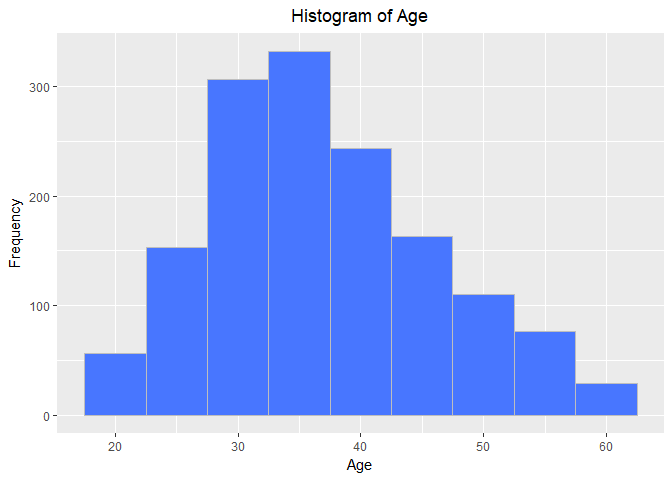
\includegraphics{Attrition_Analysis_files/figure-latex/Question 3b-1.pdf}

\begin{Shaded}
\begin{Highlighting}[]
\KeywordTok{ggplot}\NormalTok{(}\DataTypeTok{data =} \NormalTok{talentManage, }\DataTypeTok{mapping =} \KeywordTok{aes}\NormalTok{(MonthlyIncm)) +}
\StringTok{  }\KeywordTok{geom_histogram}\NormalTok{(}\DataTypeTok{binwidth =} \DecValTok{1000}\NormalTok{, }\DataTypeTok{color =} \StringTok{"gray"}\NormalTok{, }\DataTypeTok{fill =} \StringTok{"orchid3"} \NormalTok{) +}
\StringTok{  }\KeywordTok{labs}\NormalTok{(}\DataTypeTok{x =} \StringTok{"Montly income (in US$)"}\NormalTok{, }\DataTypeTok{y =} \StringTok{"Frequency"}\NormalTok{, }\DataTypeTok{title =} \StringTok{"Histogram of Monthly Income"}\NormalTok{) +}\StringTok{ }
\StringTok{  }\KeywordTok{scale_x_continuous}\NormalTok{(}\DataTypeTok{label =} \NormalTok{comma) +}
\StringTok{  }\KeywordTok{theme}\NormalTok{(}\DataTypeTok{plot.title =} \KeywordTok{element_text}\NormalTok{(}\DataTypeTok{hjust =} \FloatTok{0.5}\NormalTok{)) }
\end{Highlighting}
\end{Shaded}

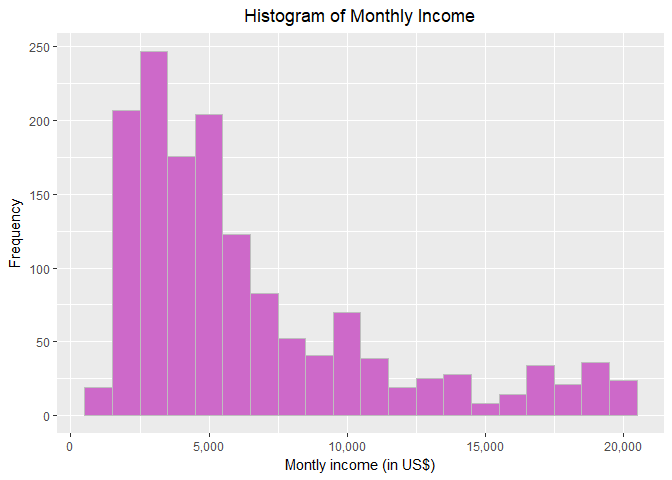
\includegraphics{Attrition_Analysis_files/figure-latex/Question 3b-2.pdf}

\textbf{c Give the frequencies (in table format or similar) for Gender,
Education, and Occupation. They can be separate tables, if that's your
choice.}

\begin{Shaded}
\begin{Highlighting}[]
\CommentTok{# Summarize categorical variables with counts}

\NormalTok{summary_factor <-}\StringTok{ }\KeywordTok{with}\NormalTok{(talentManage,}
                \KeywordTok{list}\NormalTok{(}\StringTok{"Gender"} \NormalTok{=}\StringTok{ }\KeywordTok{tab_summary}\NormalTok{(}\KeywordTok{factor}\NormalTok{(Gender)),}
                     \StringTok{"Education"} \NormalTok{=}\StringTok{ }\KeywordTok{tab_summary}\NormalTok{(}\KeywordTok{factor}\NormalTok{(Education)),}
                     \StringTok{"Ocupation"} \NormalTok{=}\StringTok{ }\KeywordTok{tab_summary}\NormalTok{(}\KeywordTok{factor}\NormalTok{(EducatinFld))))}

\NormalTok{table_factor <-}\StringTok{ }\KeywordTok{summary_table}\NormalTok{(talentManage, summary_factor)}
\NormalTok{table_factor}
\end{Highlighting}
\end{Shaded}

\begin{verbatim}
## 
## 
## |                              |talentManage (N = 1470) |
## |:-----------------------------|:-----------------------|
## |**Gender**                    |&nbsp;&nbsp;            |
## |&nbsp;&nbsp; Female           |588 (40)                |
## |&nbsp;&nbsp; Male             |882 (60)                |
## |**Education**                 |&nbsp;&nbsp;            |
## |&nbsp;&nbsp; Below College    |170 (12)                |
## |&nbsp;&nbsp; College          |282 (19)                |
## |&nbsp;&nbsp; Bachelor         |572 (39)                |
## |&nbsp;&nbsp; Master           |398 (27)                |
## |&nbsp;&nbsp; Doctor           |48 (3)                  |
## |**Ocupation**                 |&nbsp;&nbsp;            |
## |&nbsp;&nbsp; Human Resources  |27 (2)                  |
## |&nbsp;&nbsp; Life Sciences    |606 (41)                |
## |&nbsp;&nbsp; Marketing        |159 (11)                |
## |&nbsp;&nbsp; Medical          |464 (32)                |
## |&nbsp;&nbsp; Other            |82 (6)                  |
## |&nbsp;&nbsp; Technical Degree |132 (9)                 |
\end{verbatim}

\textbf{d Give the counts (again, table) of management positions.}

\begin{Shaded}
\begin{Highlighting}[]
\NormalTok{summary_positions <-}\StringTok{ }\KeywordTok{with}\NormalTok{(talentManage,}
                     \KeywordTok{list}\NormalTok{(}\StringTok{"Management Positions"} \NormalTok{=}\StringTok{ }\KeywordTok{tab_summary}\NormalTok{(}\KeywordTok{factor}\NormalTok{(JobLevel[JobLevel ==}\StringTok{ }\DecValTok{3} \NormalTok{|}\StringTok{ }\NormalTok{JobLevel ==}\DecValTok{4} \NormalTok{|}\StringTok{ }\NormalTok{JobLevel ==}\DecValTok{5}\NormalTok{]))))}

\NormalTok{table_positions <-}\StringTok{ }\KeywordTok{summary_table}\NormalTok{(talentManage, summary_positions)}
\NormalTok{table_positions}
\end{Highlighting}
\end{Shaded}

\begin{verbatim}
## 
## 
## |                         |talentManage (N = 1470) |
## |:------------------------|:-----------------------|
## |**Management Positions** |&nbsp;&nbsp;            |
## |&nbsp;&nbsp; 3           |218 (55)                |
## |&nbsp;&nbsp; 4           |106 (27)                |
## |&nbsp;&nbsp; 5           |69 (18)                 |
\end{verbatim}

\subsubsection{4. Deeper Analysis and
Visualization}\label{deeper-analysis-and-visualization}

a Note: You should make all of these appealing looking. Remember to
include things like a clean, informative title, axis labels that are in
plain English, and readable axis values that do not overlap.

b Create bar charts in ggplot or similar. The bars should be in
descending order, Use any color palette of your choice other than the
default.

c Is there a relationship between Age and Income? Create a scatterplot
and make an assessment of whether there is a relationship. Color each
point based on the Gender of the participant. You're welcome to use lm()
or similar functions to back up your claims.

d What about Life Satisfaction? Create another scatterplot. Is there a
discernible relationship there to what?


\end{document}
